\usepackage{amsthm}

\newtheorem{theorem}{Theorem}[chapter]
\newtheorem{lemma}           [theorem] {Lemma}   
\newtheorem{folg}           [theorem] {Folgerung}   

\newtheorem{frage}       [theorem] {Frage}   
\newtheorem{question}       [theorem] {Question}   
\newtheorem{aufgabe}       [theorem] {Aufgabe}   
\newtheorem{exercise}       [theorem] {Exercise}  

\newtheorem{proposition}     [theorem] {Proposition}  
\newtheorem{satz}     [theorem] {Satz}  
\newtheorem{fact}{Fact}
\newtheorem{definition}      [theorem] {Definition} 

\theoremstyle{definition} 
\newtheorem{bemerkung}     [theorem] {Bemerkung}  
\newtheorem{beispiel}       [theorem] {Beispiel}  
\newtheorem{example}       [theorem] {Example}  
\newtheorem*{example*} {Example}  
\newtheorem{notation}       [theorem] {Notation}  
\newtheorem*{Faust}[theorem]{Rule of Thumb}
\newtheorem*{Boxx}[theorem]{Concept}

\begin{Theorem}{Intermediate Value Theorem}
Let $a,b\in\mathbb{R}$ with $a<b$. Moreover, let $f:[a,b]\to\mathbb{R}$ be continuous. Let $x_0,x_1\in [a,b]$ and let $y\in\mathbb{R}$ be between $f(x_0)$ and $f(x_1)$. Then there exists some $\hat{x}$ between $x_0$ and $x_1$ such that $y=f(\hat{x})$.
\end{Theorem}

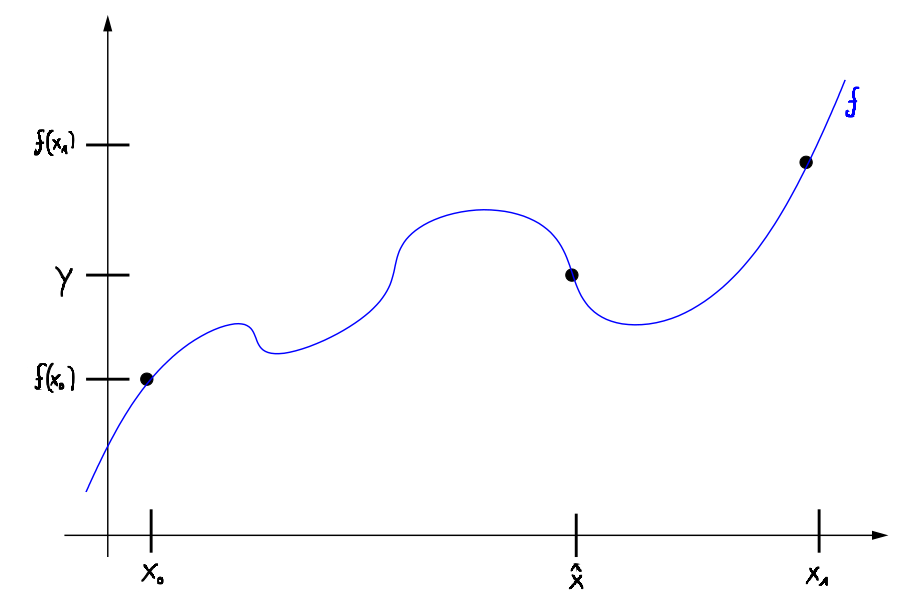
\includegraphics{./imvt.png}


\begin{proof}
Without loss of generality, we assume that $x_0<x_1$. Moreover, we can assume without loss of generality that $y=0$ (otherwise, consider the function $f(x)-y$ instead of $f$). Furthermore,
we can assume without loss of generality that $f(x_0)\leq0$ and $f(x_1)\geq0$ (otherwise, consider $-f$ instead of $f$).\\
We will construct $\hat{x}$ by nested intervals (compare the proof of the Bolzano-Weierstrass Theorem).\\
Inductively define $A_0=x_0$, $B_0=x_1$ and for $k\geq1$,
\begin{itemize}
 \item[a)] $A_k=A_{k-1}$, $B_k=\frac{A_{k-1}+B_{k-1}}2$, if $f(\frac{A_{k-1}+B_{k-1}}2)\geq0$, and
 \item[b)] $A_k=\frac{A_{k-1}+B_{k-1}}2$, $B_k=B_{k-1}$, if $f(\frac{A_{k-1}+B_{k-1}}2)\leq0$.
\end{itemize}
Then we have
\[\lim_{n\to\infty}A_n=\lim_{n\to\infty}B_n=:\hat{x}.\]
By the continuity of $f$ and the fact that $f(A_n)\leq0$, $f(B_n)\geq0$ for all $n\in\mathbb{N}$, we have
\[0\geq\lim_{n\to\infty}f(A_n)=f(\hat{x})=\lim_{n\to\infty}f(B_n)\geq0\]
and thus $f(\hat{x})=0$.
\end{proof}

